% neural_network.tex
% TikZ visualization of neural network architectures
% Demonstrates advanced TikZ techniques for drawing neural networks

\documentclass[12pt,a4paper]{article}

\usepackage{tikz}
\usepackage[margin=0.75in]{geometry}
\usepackage{amsmath}

\usetikzlibrary{positioning, calc, arrows.meta, shapes}

\title{Neural Network Visualizations with TikZ}
\author{LaTeX Student}
\date{\today}

\begin{document}

\maketitle

\section{Simple Feedforward Neural Network}

\begin{center}
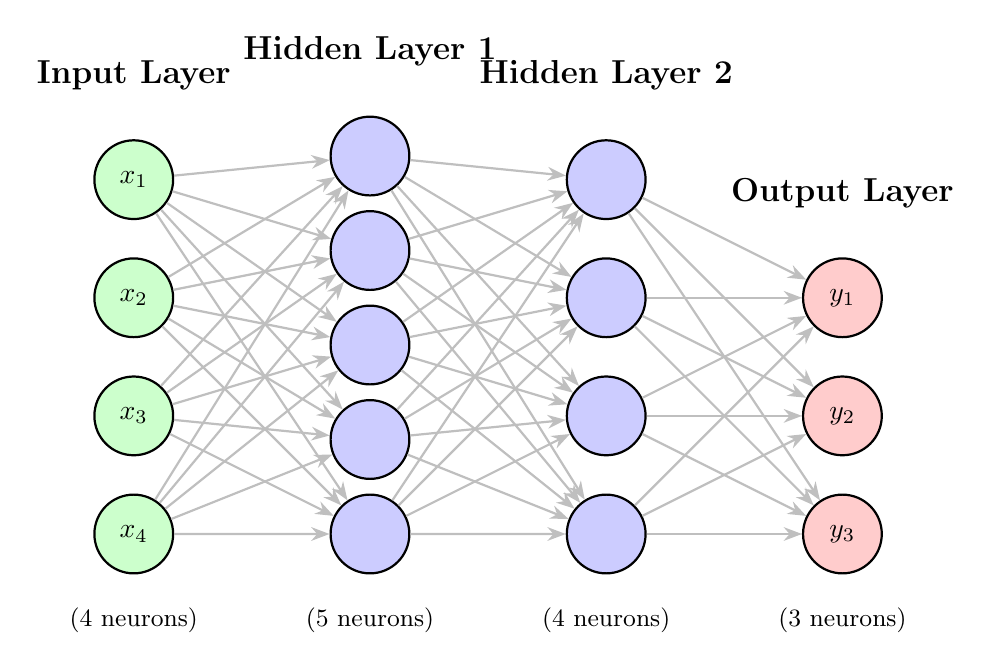
\begin{tikzpicture}[
    neuron/.style={circle, draw=black, thick, minimum size=1cm, fill=blue!20},
    input/.style={circle, draw=black, thick, minimum size=1cm, fill=green!20},
    output/.style={circle, draw=black, thick, minimum size=1cm, fill=red!20},
    arrow/.style={->,>=Stealth, thick}
]

    % Input layer
    \foreach \i in {1,2,3,4} {
        \node[input] (I\i) at (0, -\i*1.5) {$x_\i$};
    }

    % Hidden layer 1
    \foreach \i in {1,2,3,4,5} {
        \node[neuron] (H1\i) at (3, -\i*1.2) {};
    }

    % Hidden layer 2
    \foreach \i in {1,2,3,4} {
        \node[neuron] (H2\i) at (6, -\i*1.5) {};
    }

    % Output layer
    \foreach \i in {1,2,3} {
        \node[output] (O\i) at (9, {-1.5-\i*1.5}) {$y_\i$};
    }

    % Connections: Input to Hidden1
    \foreach \i in {1,2,3,4} {
        \foreach \j in {1,2,3,4,5} {
            \draw[arrow, gray!50] (I\i) -- (H1\j);
        }
    }

    % Connections: Hidden1 to Hidden2
    \foreach \i in {1,2,3,4,5} {
        \foreach \j in {1,2,3,4} {
            \draw[arrow, gray!50] (H1\i) -- (H2\j);
        }
    }

    % Connections: Hidden2 to Output
    \foreach \i in {1,2,3,4} {
        \foreach \j in {1,2,3} {
            \draw[arrow, gray!50] (H2\i) -- (O\j);
        }
    }

    % Layer labels
    \node[above=0.5cm of I1, font=\large\bfseries] {Input Layer};
    \node[above=0.5cm of H11, font=\large\bfseries] {Hidden Layer 1};
    \node[above=0.5cm of H21, font=\large\bfseries] {Hidden Layer 2};
    \node[above=0.5cm of O1, font=\large\bfseries] {Output Layer};

    % Dimension annotations
    \node[below=0.3cm of I4, font=\small] {(4 neurons)};
    \node[below=0.3cm of H15, font=\small] {(5 neurons)};
    \node[below=0.3cm of H24, font=\small] {(4 neurons)};
    \node[below=0.3cm of O3, font=\small] {(3 neurons)};

\end{tikzpicture}
\end{center}

\section{Convolutional Neural Network (CNN)}

\begin{center}
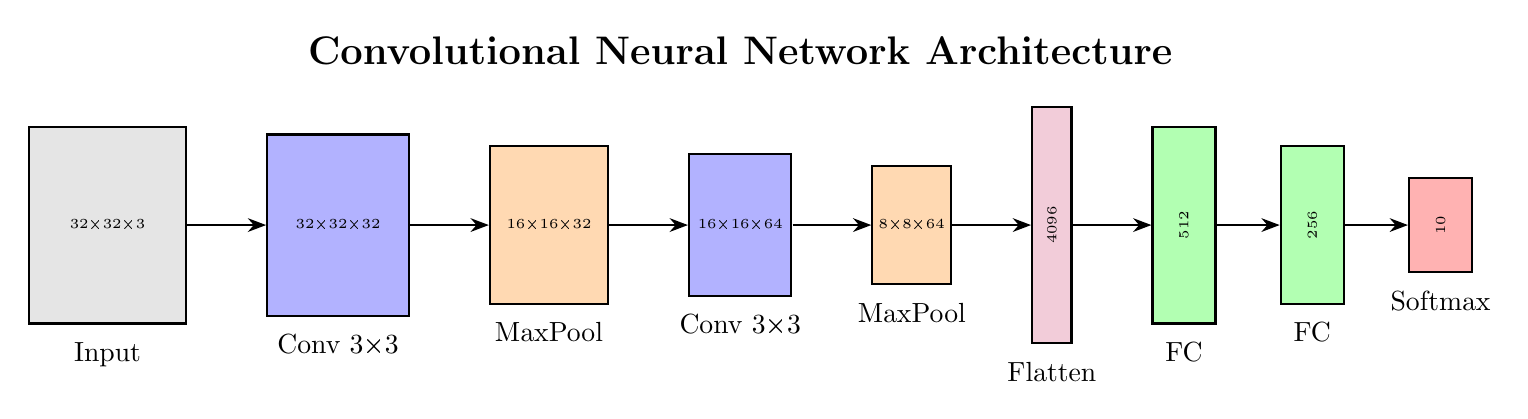
\begin{tikzpicture}[
    scale=0.8,
    layer/.style={rectangle, draw=black, thick, minimum width=1.5cm, minimum height=2cm},
    conv/.style={layer, fill=blue!30},
    pool/.style={layer, fill=orange!30},
    fc/.style={layer, fill=green!30, minimum width=0.8cm, minimum height=1.5cm},
    arrow/.style={->,>=Stealth, thick}
]

    % Input
    \node[layer, fill=gray!20, minimum width=2cm, minimum height=2.5cm] (input) at (0,0) {};
    \node[below=0.1cm of input] {Input};
    \node[font=\tiny] at (input.center) {32×32×3};

    % Conv1
    \node[conv, right=1cm of input, minimum width=1.8cm, minimum height=2.3cm] (conv1) {};
    \node[below=0.1cm of conv1] {Conv 3×3};
    \node[font=\tiny] at (conv1.center) {32×32×32};

    % Pool1
    \node[pool, right=1cm of conv1, minimum width=1.5cm, minimum height=2cm] (pool1) {};
    \node[below=0.1cm of pool1] {MaxPool};
    \node[font=\tiny] at (pool1.center) {16×16×32};

    % Conv2
    \node[conv, right=1cm of pool1, minimum width=1.3cm, minimum height=1.8cm] (conv2) {};
    \node[below=0.1cm of conv2] {Conv 3×3};
    \node[font=\tiny] at (conv2.center) {16×16×64};

    % Pool2
    \node[pool, right=1cm of conv2, minimum width=1cm, minimum height=1.5cm] (pool2) {};
    \node[below=0.1cm of pool2] {MaxPool};
    \node[font=\tiny] at (pool2.center) {8×8×64};

    % Flatten
    \node[layer, fill=purple!20, right=1cm of pool2, minimum width=0.5cm, minimum height=3cm] (flatten) {};
    \node[below=0.1cm of flatten] {Flatten};
    \node[font=\tiny, rotate=90] at (flatten.center) {4096};

    % FC1
    \node[fc, right=1cm of flatten, minimum height=2.5cm] (fc1) {};
    \node[below=0.1cm of fc1] {FC};
    \node[font=\tiny, rotate=90] at (fc1.center) {512};

    % FC2
    \node[fc, right=0.8cm of fc1, minimum height=2cm] (fc2) {};
    \node[below=0.1cm of fc2] {FC};
    \node[font=\tiny, rotate=90] at (fc2.center) {256};

    % Output
    \node[fc, right=0.8cm of fc2, minimum height=1.2cm, fill=red!30] (output) {};
    \node[below=0.1cm of output] {Softmax};
    \node[font=\tiny, rotate=90] at (output.center) {10};

    % Arrows
    \draw[arrow] (input) -- (conv1);
    \draw[arrow] (conv1) -- (pool1);
    \draw[arrow] (pool1) -- (conv2);
    \draw[arrow] (conv2) -- (pool2);
    \draw[arrow] (pool2) -- (flatten);
    \draw[arrow] (flatten) -- (fc1);
    \draw[arrow] (fc1) -- (fc2);
    \draw[arrow] (fc2) -- (output);

    % Title
    \node[above=1cm of conv2, font=\Large\bfseries] {Convolutional Neural Network Architecture};

\end{tikzpicture}
\end{center}

\section{Recurrent Neural Network (RNN)}

\begin{center}
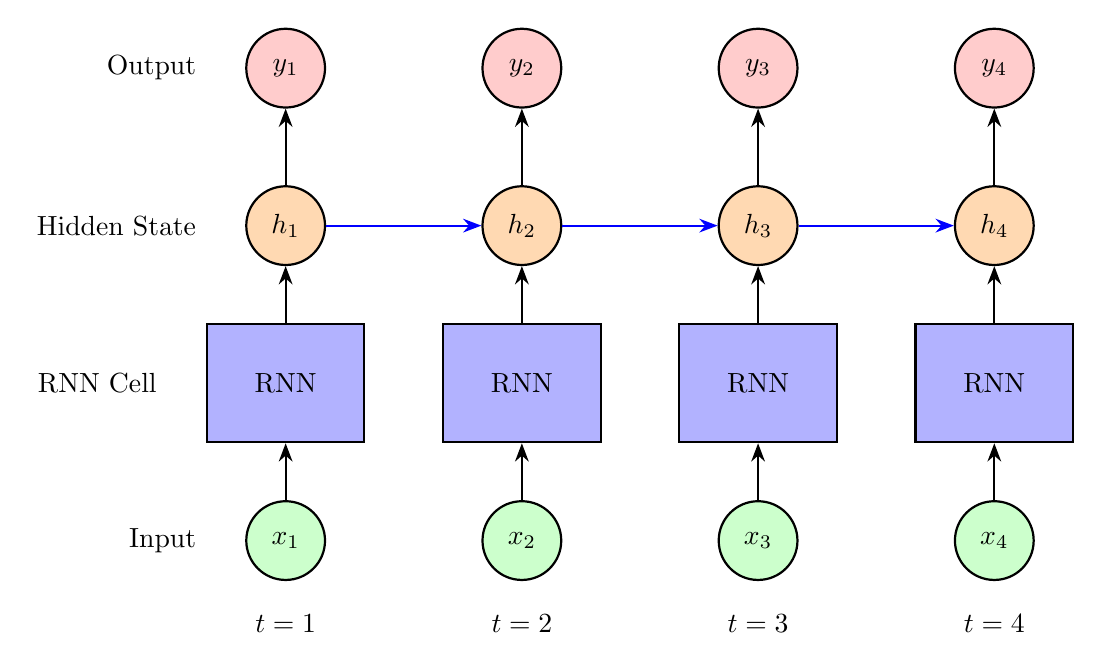
\begin{tikzpicture}[
    node distance=2cm,
    rnn/.style={rectangle, draw=black, thick, minimum width=2cm, minimum height=1.5cm, fill=blue!30},
    state/.style={circle, draw=black, thick, minimum size=1cm, fill=orange!30},
    arrow/.style={->,>=Stealth, thick}
]

    % Time steps
    \foreach \t in {1,2,3,4} {
        % Input
        \node[state, fill=green!20] (x\t) at (\t*3, 0) {$x_\t$};

        % RNN cell
        \node[rnn] (rnn\t) at (\t*3, 2) {RNN};

        % Hidden state
        \node[state] (h\t) at (\t*3, 4) {$h_\t$};

        % Output
        \node[state, fill=red!20] (y\t) at (\t*3, 6) {$y_\t$};

        % Vertical connections
        \draw[arrow] (x\t) -- (rnn\t);
        \draw[arrow] (rnn\t) -- (h\t);
        \draw[arrow] (h\t) -- (y\t);
    }

    % Horizontal connections (hidden states)
    \foreach \t in {1,2,3} {
        \pgfmathtruncatemacro{\next}{\t+1}
        \draw[arrow, blue, thick] (h\t) -- (h\next);
    }

    % Labels
    \node[left=0.5cm of x1] {Input};
    \node[left=0.5cm of rnn1] {RNN Cell};
    \node[left=0.5cm of h1] {Hidden State};
    \node[left=0.5cm of y1] {Output};

    \node[below=0.3cm of x1] {$t=1$};
    \node[below=0.3cm of x2] {$t=2$};
    \node[below=0.3cm of x3] {$t=3$};
    \node[below=0.3cm of x4] {$t=4$};

\end{tikzpicture}
\end{center}

\section{LSTM Cell Architecture}

\begin{center}
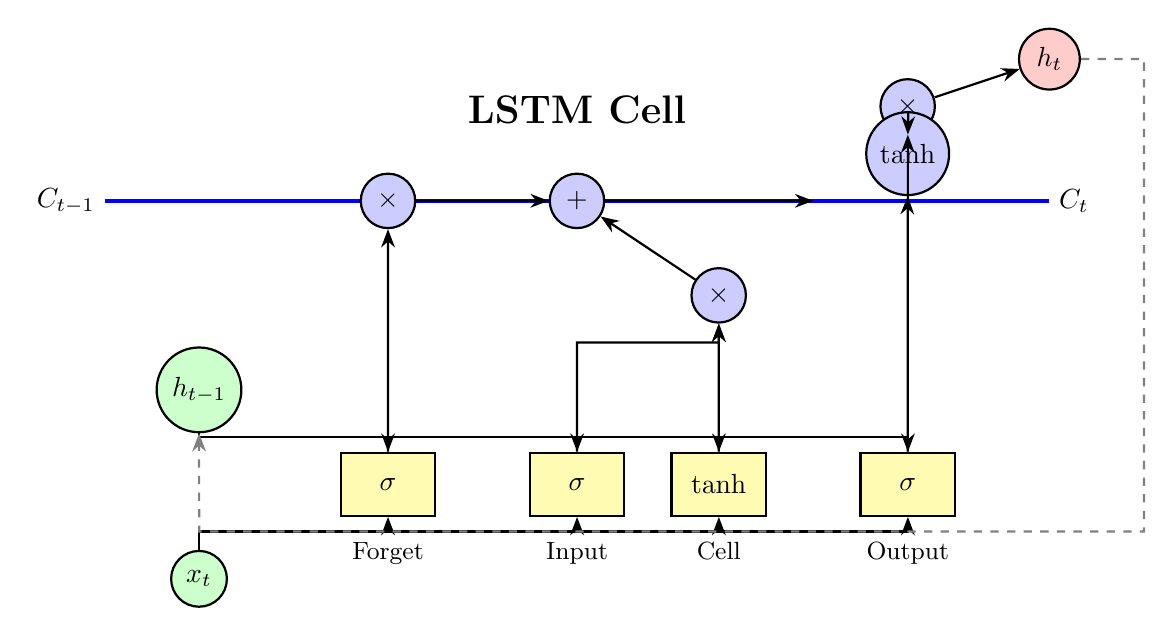
\begin{tikzpicture}[
    scale=1.2,
    gate/.style={rectangle, draw=black, thick, minimum width=1.2cm, minimum height=0.8cm, fill=yellow!30},
    operation/.style={circle, draw=black, thick, minimum size=0.6cm, fill=blue!20},
    arrow/.style={->,>=Stealth, thick}
]

    % Input and previous hidden state
    \node[operation, fill=green!20] (x) at (0, 0) {$x_t$};
    \node[operation, fill=green!20] (h_prev) at (0, 2) {$h_{t-1}$};

    % Cell state
    \draw[ultra thick, blue] (-1, 4) -- (9, 4);
    \node[left] at (-1, 4) {$C_{t-1}$};
    \node[right] at (9, 4) {$C_t$};

    % Gates
    \node[gate] (forget) at (2, 1) {$\sigma$};
    \node[below=0.2cm of forget, font=\small] {Forget};

    \node[gate] (input_gate) at (4, 1) {$\sigma$};
    \node[below=0.2cm of input_gate, font=\small] {Input};

    \node[gate] (cell_gate) at (5.5, 1) {$\tanh$};
    \node[below=0.2cm of cell_gate, font=\small] {Cell};

    \node[gate] (output_gate) at (7.5, 1) {$\sigma$};
    \node[below=0.2cm of output_gate, font=\small] {Output};

    % Operations
    \node[operation] (mult1) at (2, 4) {$\times$};
    \node[operation] (mult2) at (5.5, 3) {$\times$};
    \node[operation] (add) at (4, 4) {$+$};
    \node[operation] (mult3) at (7.5, 5) {$\times$};
    \node[operation] (tanh_out) at (7.5, 4.5) {$\tanh$};

    % Output
    \node[operation, fill=red!20] (h) at (9, 5.5) {$h_t$};

    % Connections from inputs
    \draw[arrow] (x) -- ++(0, 0.5) -| (forget);
    \draw[arrow] (x) ++(0, 0.5) -| (input_gate);
    \draw[arrow] (x) ++(0, 0.5) -| (cell_gate);
    \draw[arrow] (x) ++(0, 0.5) -| (output_gate);

    \draw[arrow] (h_prev) -- ++(0, -0.5) -| (forget);
    \draw[arrow] (h_prev) ++(0, -0.5) -| (input_gate);
    \draw[arrow] (h_prev) ++(0, -0.5) -| (cell_gate);
    \draw[arrow] (h_prev) ++(0, -0.5) -| (output_gate);

    % Gate to operations
    \draw[arrow] (forget) -- (mult1);
    \draw[arrow] (input_gate) -- ++(0, 1.5) -| (mult2);
    \draw[arrow] (cell_gate) -- (mult2);
    \draw[arrow] (output_gate) -- ++(0, 3) -| (mult3);

    % Cell state operations
    \draw[arrow] (mult1) -- (add);
    \draw[arrow] (mult2) -- (add);
    \draw[arrow] (add) -- ++(2.5, 0);

    % Output path
    \draw[arrow] (7.5, 4) -- (tanh_out);
    \draw[arrow] (tanh_out) -- (mult3);
    \draw[arrow] (mult3) -- (h);

    % Output feedback
    \draw[arrow, dashed, gray] (h) -- ++(1, 0) -- ++(0, -5) -- ++(-10, 0) -- (h_prev);

    % Title
    \node[above=0.5cm of add, font=\Large\bfseries] {LSTM Cell};

\end{tikzpicture}
\end{center}

\section{Autoencoder Architecture}

\begin{center}
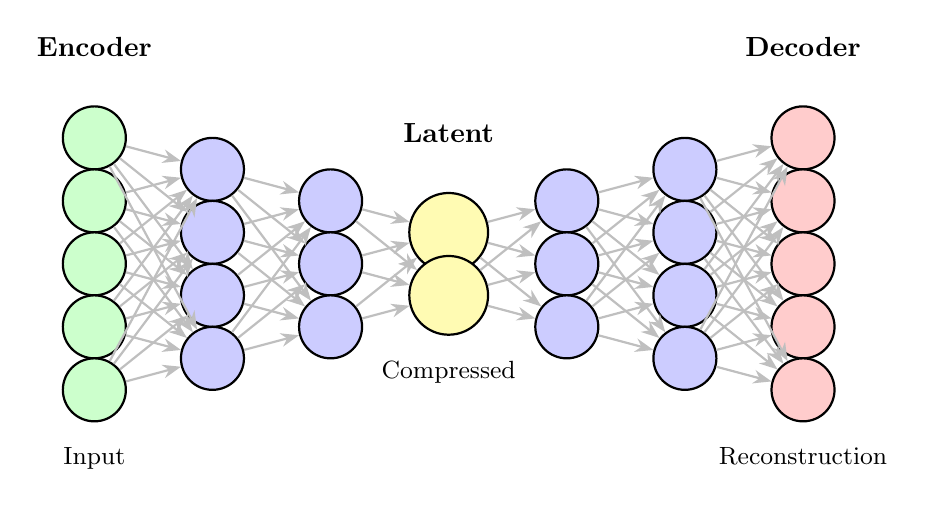
\begin{tikzpicture}[
    node distance=1.5cm,
    layer/.style={circle, draw=black, thick, minimum size=0.8cm, fill=blue!20},
    arrow/.style={->,>=Stealth, thick, gray!50}
]

    % Encoder
    \foreach \i in {1,...,5} {
        \node[layer, fill=green!20] (e0-\i) at (0, -\i*0.8) {};
    }

    \foreach \i in {1,...,4} {
        \node[layer] (e1-\i) at (1.5, {-0.4-\i*0.8}) {};
    }

    \foreach \i in {1,...,3} {
        \node[layer] (e2-\i) at (3, {-0.8-\i*0.8}) {};
    }

    % Latent space
    \foreach \i in {1,2} {
        \node[layer, fill=yellow!30, minimum size=1cm] (latent-\i) at (4.5, {-1.2-\i*0.8}) {};
    }

    % Decoder
    \foreach \i in {1,...,3} {
        \node[layer] (d1-\i) at (6, {-0.8-\i*0.8}) {};
    }

    \foreach \i in {1,...,4} {
        \node[layer] (d2-\i) at (7.5, {-0.4-\i*0.8}) {};
    }

    \foreach \i in {1,...,5} {
        \node[layer, fill=red!20] (d3-\i) at (9, -\i*0.8) {};
    }

    % Connections (simplified - not all connections shown)
    \foreach \i in {1,...,5} {
        \foreach \j in {1,...,4} {
            \draw[arrow] (e0-\i) -- (e1-\j);
        }
    }

    \foreach \i in {1,...,4} {
        \foreach \j in {1,...,3} {
            \draw[arrow] (e1-\i) -- (e2-\j);
        }
    }

    \foreach \i in {1,...,3} {
        \foreach \j in {1,2} {
            \draw[arrow] (e2-\i) -- (latent-\j);
        }
    }

    \foreach \i in {1,2} {
        \foreach \j in {1,...,3} {
            \draw[arrow] (latent-\i) -- (d1-\j);
        }
    }

    \foreach \i in {1,...,3} {
        \foreach \j in {1,...,4} {
            \draw[arrow] (d1-\i) -- (d2-\j);
        }
    }

    \foreach \i in {1,...,4} {
        \foreach \j in {1,...,5} {
            \draw[arrow] (d2-\i) -- (d3-\j);
        }
    }

    % Labels
    \node[above=0.5cm of e0-1, font=\bfseries] {Encoder};
    \node[above=0.5cm of latent-1, font=\bfseries] {Latent};
    \node[above=0.5cm of d3-1, font=\bfseries] {Decoder};

    \node[below=0.2cm of e0-5, font=\small] {Input};
    \node[below=0.2cm of latent-2, font=\small] {Compressed};
    \node[below=0.2cm of d3-5, font=\small] {Reconstruction};

\end{tikzpicture}
\end{center}

\section{Compilation Notes}

To compile this document:
\begin{verbatim}
pdflatex neural_network.tex
\end{verbatim}

For complex networks with many neurons, consider using loops and
programmatic approaches to reduce code duplication.

\end{document}
